\begin{columns}[totalwidth=.85\linewidth]
	\column{\textwidth}
	\vspace{-10mm}
		% \begin{boxnote}
		% 	\textbf{高分子材料でマルチマテリアル化 $\Leftrightarrow$ 高い比強度の有効利用}
        %         \begin{itemize}
        %             \item 高分子材料の破壊耐性向上の設計指針を得たい。
        %             \item 耐久性、可逆性に優れた材料としてゴム材料を選択
        %         \end{itemize}
		% 	\textbf{アプローチ}
		% 		\begin{itemize}
		% 			% \item 実験的アプローチ
		% 			% \begin{itemize}
		% 			% 	\normalsize
		% 			% 	\item 構造明確な\alert{三分岐}ネットワークを超分子で構築
		% 			% 	\item フィラー無添加での\alert{高い破断伸びと強度}
		% 			% 	\item 既知のモデルとの多数の整合点と、\alert{よくわからない点}。
		% 			% \end{itemize}
		% 			\item マルチスケールシミュレーションで\color{red}モデル\color{black}を構築
		% 			\begin{itemize}
		% 				\normalsize
		% 				\item 単純化したモデルで小さなスケールから始めたい。
		% 				\item \alert{長さの揃ったストランドで MD シミュレーション}
		% 				% \item 最終的に、亀裂先端の挙動を FEM シミュレーション
		% 			\end{itemize}
		% 		\end{itemize}
		% \end{boxnote}

		% \begin{itembox}[l]{古典ゴム弾性理論でのミクロな変形モデル}
		% 	\begin{columns}[T, onlytextwidth]
		% 		\column{.48\linewidth}
		% 			\begin{itembox}[l]{Affine Network Model}
		% 				\begin{itemize}
		% 					\item 架橋点の Affine 変形を仮定
		% 						\begin{align*}
		% 							\sigma_{nom} &= \textcolor{red}{\nu} k_B T \left(\lambda - \dfrac{1}{\lambda^2}\right) \\
		% 							&= G_{affine} \left(\lambda - \dfrac{1}{\lambda^2}\right)
		% 						\end{align*}
		% 				\end{itemize}
		% 			\end{itembox}
		% 		\column{.48\linewidth}
		% 			\begin{itembox}[l]{Phantom Network Model}
		% 				\begin{itemize}
		% 					\item \alert{架橋点ゆらぎ}を考慮
		% 					\item 架橋点の分岐数 $f$
		% 				\end{itemize}
		% 				% \vspace{-2mm}
		% 				% \small
		% 				\begin{align*}
		% 					G_{phantom} &= \nu k_B T \left(1 - \dfrac{2}{f}\right) \\
		% 				\end{align*}
		% 			\end{itembox}
		% 	\end{columns}     
		% \end{itembox}



		\begin{itembox}[l]{Classical Theory of Rubber Elasticity}
			% \begin{block}{Free Energy Density of Rubbers against Strain invariant}
			% 	\vspace{-2mm}
				% 非圧縮性条件から第3不変量がおちて、
				Free Energy Density of Rubbers against Strain Invariant
				\small
				\begin{align*}
					\dfrac{F}{V} = W 
					% &= \sum_{i,j = 0}^{\infty} C_{ij}(I_1-3)^i(I_2-3)^j \\[-2mm]
					&= C_0 + \underbrace{{\color{green}C_1(I_1-3)} + {\color{red}C_2(I_2-3)}}_{\color{red}Mooney-Rivlin Model} + \sum_{i,j = 1}^{\infty} C_{ij}(I_1-3)^i(I_2-3)^j
				\end{align*}  
			% \end{block}
			% \vspace{-5mm}
			\begin{columns}[T, onlytextwidth]
				\column{.48\linewidth}
					\begin{itembox}{Neo-Hookean Model}
						% \vspace{-2mm}
						% 第1不変量のみを対象
							\small
							\begin{align*}
								&W = C_1 (I_1-3) \\
								&\text{against Uniaxial elongation} \\
								&\sigma_{nom} = 2 C_1\left(\lambda - \dfrac{1}{\lambda^2}\right) = G \left(\lambda - \dfrac{1}{\lambda^2}\right)
							\end{align*}
					\end{itembox}
				\column{.48\linewidth}
					\begin{itembox}{Mooney-Rivlin Model}
						% \vspace{-2mm}
						% 高次の項をおとす
						\small
						\begin{align*}
							&W = C_1 (I_1-3) + C_2(I_2-3) \\
							&\text{against Uniaxial elongation} \\
							&\sigma_{nom} = 2 \left(C_1 + C_2\dfrac{1}{\lambda} \right) \left(\lambda - \dfrac{1}{\lambda^2}\right)
						\end{align*}
					\end{itembox}
			\end{columns}
			% \vspace{-1mm}
			\begin{itembox}{With or without Junction Poinits fluctuation}
				\vspace{3mm}
				\begin{columns}[T, onlytextwidth]
					\column{.45\linewidth}
					% \small
					\color{blue}{Affine Network Model
					% \footnote{
					% 	\tiny{P.J. Flory, Principles of Polymer Chemistry, (1953)}
					% }
					}
					% \vspace{-2mm}
					\small
					\begin{align*}
						% &\text{Affine Network Model}\\
						&G_{affine} = \nu k_B T  \\
						&\text{$\nu$: Number density of strands}
					\end{align*}
					\column{.45\linewidth}
					% \small
					\color{red}{Phantom Network Model
					% \footnote{
					% 	\tiny{H.M. James, E.J. Guth, Chem. Phys., 21, 6, 1039 (1953)}
					% }
					}
					% \vspace{-2mm}
					\small
					\begin{align*}
						% &\text{Phantom Network Model}\\
						&G_{phantom} = \nu k_B T \left(1 - \dfrac{2}{f}\right) \\
						&\text{$f$: Functionality of Junction Points}
					\end{align*}
					\normalsize
				\end{columns}
			\end{itembox}

		\end{itembox}


	\begin{itembox}[l]{Recent approach for Constraints (Entanglements)}
		\begin{itemize}
			\item Diffused-Constraint Model
			\begin{itemize}
				\normalsize
				\item Confining potential affect all points along the chain.
				% \footnote{\tiny{A. Kloczkowski, J.E. Mark, B. Erman, Macromol., 28, 5089 (1995)}}
			\end{itemize}
			\item Nonaffine Tube Model
			\begin{itemize}
				\normalsize
				\item Improved model of "Edwards' Tube Model".
				% \footnote{\tiny{M. Rubinstein, S. Panyukov, Macromol., 30, 25, 8036 (1997)}}
			\end{itemize}
			\item Slip-tube Model
			\begin{itemize}
				\normalsize
				\item A pairwise interaction of chains is introduced.
				% \footnote{\tiny{M. Rubinstein, S. Panyukov, Macromol., 35, 6670 (2002)}}
			\end{itemize}
		\end{itemize}
	
		\begin{columns}[totalwidth=1\textwidth]
			\column{.65\textwidth}
			\small
			\begin{align*}
				&f^*(\lambda^{-1}) = G_c + \dfrac{G_e}{0.74 \lambda + 0.61 \lambda^{-1/2} - 0.35} \\
				&G_c = \nu k_B T \left(1-\dfrac{2}{\phi} \right), \quad G_e = \dfrac{4}{7} \nu k_B T L \\
				% &\text{where $\nu$ is the number density of network chains,} \\
				& \text{L is the number of slip-links per network chain}
			\end{align*}
			\column{.3\textwidth}
			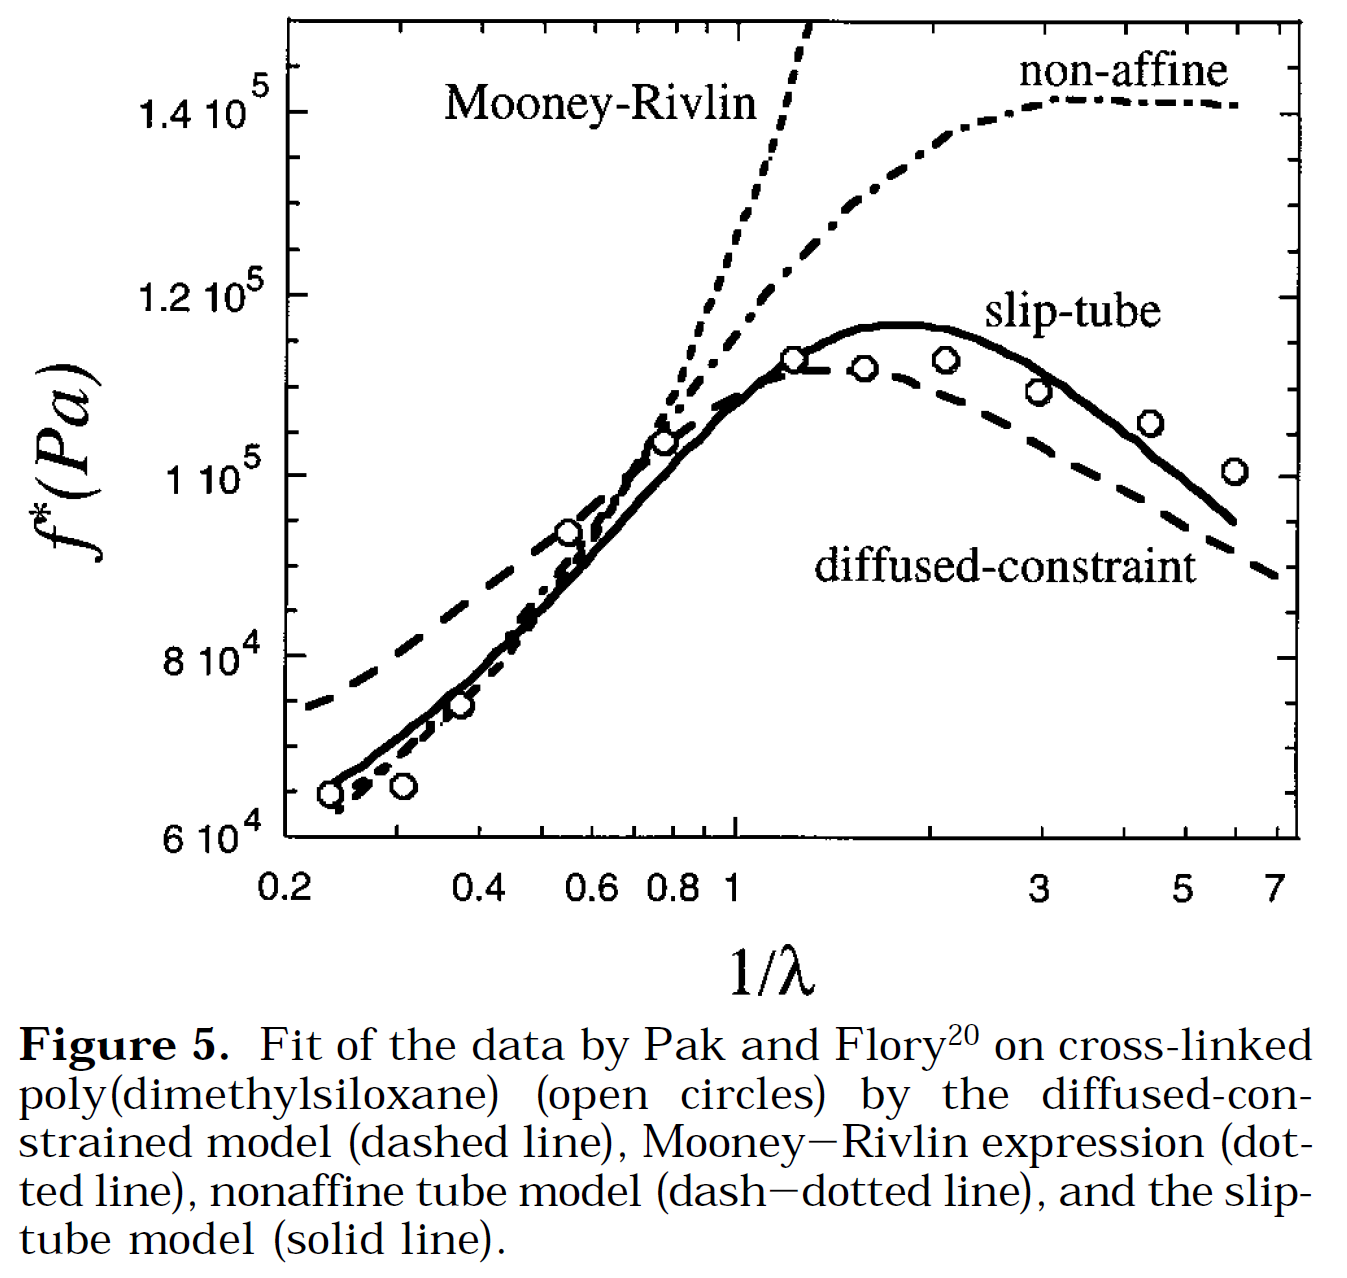
\includegraphics[width=.9\textwidth]{NW_model_rubinstein.png}
		\end{columns}
	\end{itembox}

	\begin{itembox}[l]{架橋点の環境とランダムな接続性\cite{flory}}
		\begin{columns}[totalwidth=\textwidth]
			% \column{.35\textwidth}
			% \centering
			% 	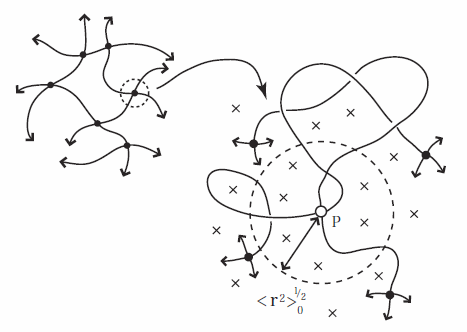
\includegraphics[width=.8\textwidth]{JP_vicinity.png}

			% 	\small
			% 	架橋点は\alert{多数のストランド}に\\囲まれている。
			\column{.6\textwidth}
				\begin{itemize}
					\item 規則構造を初期構造とする
					\begin{itemize}
						\normalsize
						\item ストランドの長さを揃える
					\end{itemize}
					\item 接続性を不均一に
						\begin{itemize}
							\normalsize
							\item 接続に\alert{位置依存性}
						\end{itemize}
					\item 巨視的な変形後
						\begin{itemize}
							\normalsize
							\item \alert{結節点のゆらぎが不均一}
							\item 多様な緩和モード
							% \item \alert{緩和の長時間化?}
						\item \alert{Phantom Network の諸特性が発現}
						\end{itemize}
				\end{itemize}
			\column{.35\textwidth}
				\centering
				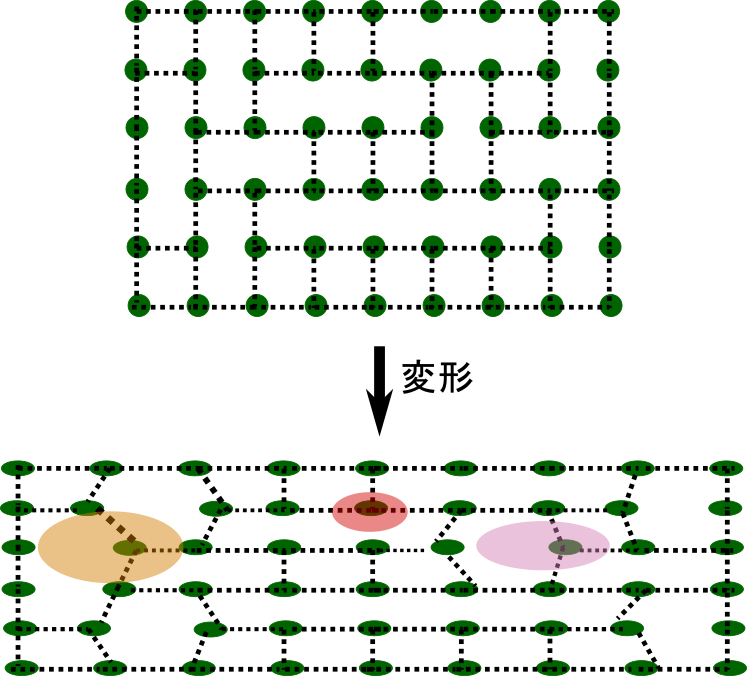
\includegraphics[width=\textwidth]{random_NW.png}
		\end{columns}
	\end{itembox}
\end{columns}